\section{Metodología}
\subsection{Solución matemática}

Un método de resolución es mediante un arreglo matricial. Considerese el sistema de ecuaciones mostrado en \ref{eq:state-equation}, se puede formar una matriz tridiagonal $M$ definida como en \ref{eq:matrix-def}, donde $\delta$ se define como $\delta_{i,j} = 1, \text{si i = j}$.

\begin{equation}
	M_{ij} = \frac{D}{\sqrt{m_i m_j}} (2 \delta_{ij} - \delta_{i, j+1} - \delta_{i, j-1}) 
	\label{eq:matrix-def}
\end{equation}

Esta representación de arreglo es plateada como alternativa de solución en la descripción del problema para este proyecto. En ese sentido, se conoce que el cálculo de las vibraciones del sistema se puede reducir al cálculo de los valores propios y vectores propios de la matriz tridiagonal. Se asume que dado el arreglo $M$, sus valores propios ($\lambda_i)$ y vectores propios $v_i$ pueden reemplazarse directamente en \ref{eq:state-equation}. Sea la ecuación \ref{eq:analytical-solution} la solución del sistema a partir del uso de los valores y vectores propios de $M$. 

\begin{equation}
	y_{i} = \sum^{n}_{i=0} v_i \cos(\lambda_i t ) + v_i \sin(\lambda_i t )  
	\label{eq:analytical-solution}
\end{equation}

\subsection{Código}
\subsubsection{Código general}

Para la obtención de los valores y vectores propios, se usa el método Tridiagonal Quadratic Linear Implicit (tqli). El algoritmo funciona para una matriz simétrica tridiagonal, por lo que propone utilizar un método de tridiagonalización utilizando un algoritmo tred2. Sin embargo, particularmente el modelo definido $M$ es simétrica tridiagonal. Por ello, se corrieron ambas opciones que considera el uso de tred2. Por conveniencia y seguir lo recomendado por la funcion, se utilizo tred2. Estas recomendaciones fueron extraídas del libro Numerical Recipes \cite{press2007numerical}. Como se puede apreciar, esta función no puede ser paralelizada a simple vista, por la presencia de bucles \textbf{while} y declaraciones \textbf{break}. 

El codigo implementado sigue el siguiente pseudocodigo mostrado en la Figura \ref{fig:pseudo}. 

\begin{figure}[htbp]
	\centering
	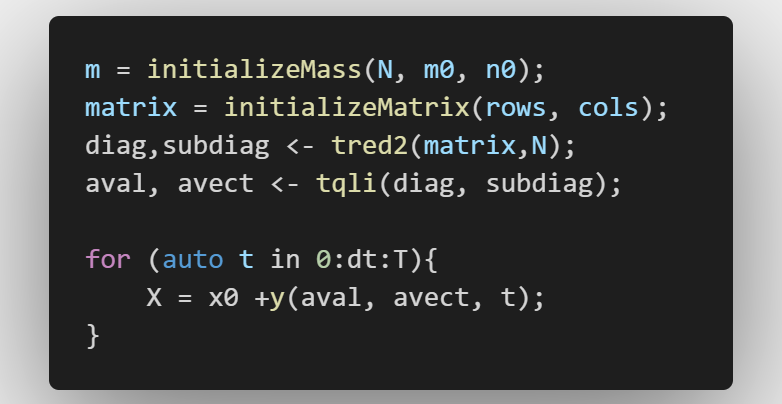
\includegraphics[width=0.45\textwidth]{pseudocode.png}
	\caption{Pseudocódigo del cóidigo implementado.}
	\label{fig:pseudo}
\end{figure}

% \begin{verbatim}
% 	m = initializeMass(n, m0, n0);
% 	matrix = initializeMatrix(n, n);
% 	diag, subdiag <- tred2(matrix, n);
% 	aval, avect <- tqli(diag, subdiag);
% 	// Simulation
% 	for t in 0:dT:T
% 		X = X0 + y(aval, avect, t);
% \end{verbatim}

Las variaciones realizadas y es donde se midio el desempeño del codigo es para la función tqli, que además de haber sido modificado del libro, se ha paralelizado mediante OpenMP \cite{al2017parallel}.


\subsubsection{Código paralelo}
Particularmente para la implementación en paralelo, se tuvo que modificar el código original. OpenMP no es compatible para statements break o while, los cuales aparecían varias veces en el código. Por lo tanto, estas secciones se modificaron para que puedan utilizarse solo for y if statements. Se registró cuáles eran las secciones no paralelizables y las que tenían mayor recurrencia en el código. Converientemente, la sección principal más recurrente, es compatible con paralelismo mediante el statement \#pragma-for. 

Respecto al resto del código, cabe resaltar que gran parte del código se basa en condicionales de forma break que interrupen el código. Además, hay recursividad en algunas variables, lo cual no puede ser manejado adecuadamente con OpenMP, a menos que se modifique la forma del algoritmo, por lo que escapó del objetivo a realizarse. Estos segmentos de código pueden apreciarse en las Figuras \ref{fig:code1}, \ref{fig:code2}, \ref{fig:code3}, \ref{fig:code4}. Pese a ello, se resalta nuevamente que la sección del código con más recurrencia sí ha sido paralelizado.


\begin{figure}
	\centering
	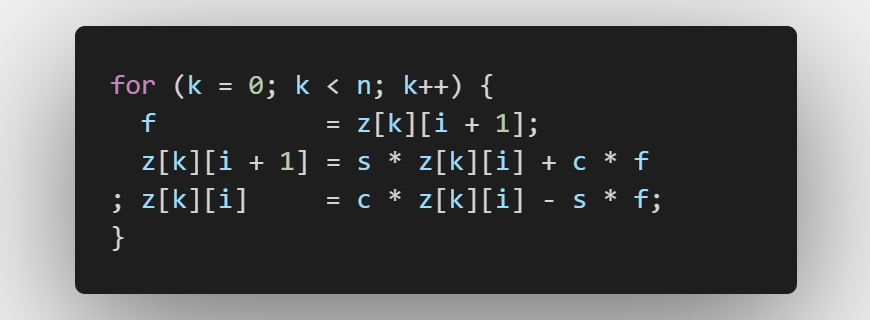
\includegraphics[width=0.45\textwidth]{code1.png}
	\caption{Fragmento de código 1.}
	\label{fig:code1}
\end{figure}

\begin{figure}
	\centering
	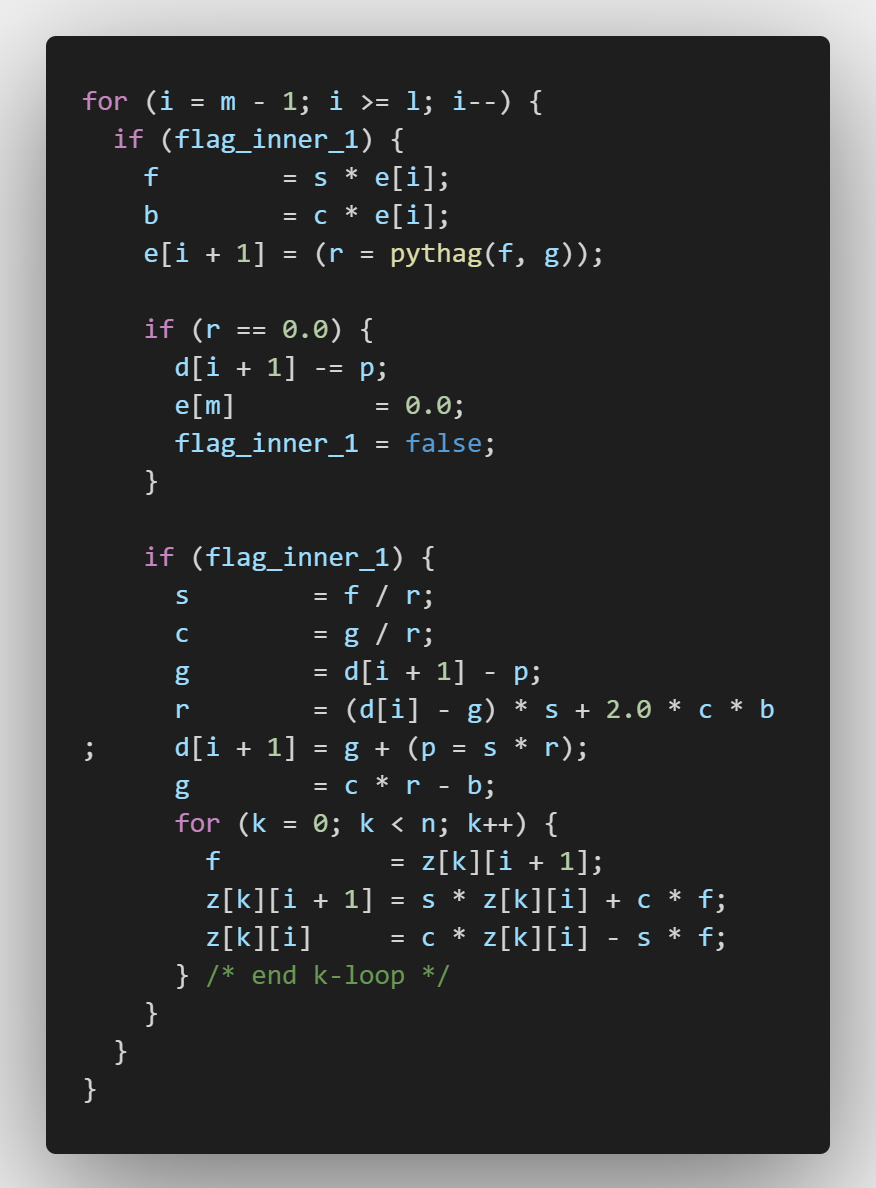
\includegraphics[width=0.45\textwidth]{code2.png}
	\caption{Fragmento de código 2.}
	\label{fig:code2}
\end{figure}


\begin{figure}
	\centering
	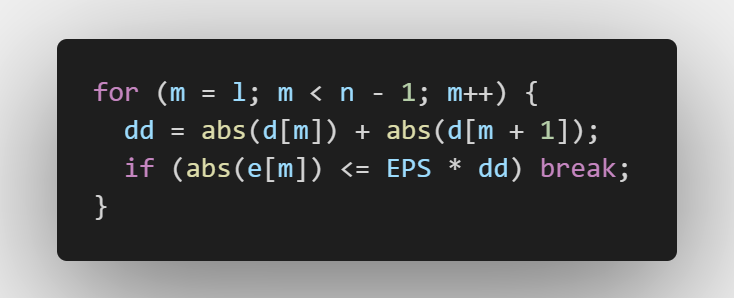
\includegraphics[width=0.45\textwidth]{code3.png}
	\caption{Fragmento de código 3.}
	\label{fig:code3}
\end{figure}

\begin{figure}
	\centering
	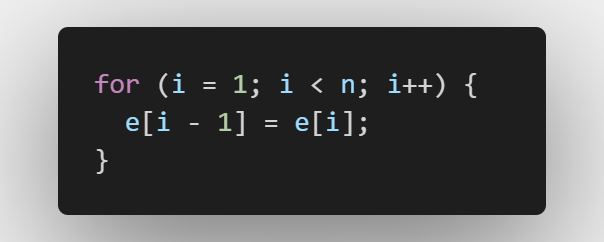
\includegraphics[width=0.45\textwidth]{code4.png}
	\caption{Fragmento de código 4.}
	\label{fig:code4}
\end{figure}

Estos fragmentos de código presentan diversos factores que no permiten una paralelización normal con OpenMP, tal como la comunicación necesaria con la memoria adyacente para cada iteración, ya se adelante a otras con un índice +1 o -1.

\subsubsection{Implementación}
El código realizado sigue el control de versiones \text{git} y se muestra en el siguiente repositorio en Github \textit{https://github.com/jhonatanmacazana/parallel-computing-project}. Notese el historial y la linea de commits realizados conjunto los releases.

Se plantearon dos tipos de experimentos para revisar el comportamiento del sistema. Para el primer caso, se plantea revisar el comportamiento por un tiempo $T = 10s$, para un $m_i = 1 kg$, excepto para un $n_0 = 30, 60$, donde $m_{n_0} = 100 kg$. El comportamiento en tiempo, se analizará posteriormente. Para el segundo lugar, se correrá el código para medir su desempeño. Se plantea correr 10 veces el código para $n={59,69,79,89,99}$. Para el caso en paralelo, se correrá el código para $p={2,4,6,8}$. Todos estos casos se correrán de manera local, en el cluster proporcionado por UTEC y en un servidor propio para benchmarking.

Para agilizar el desarrollo y poder compilar en diferentes entornos de manera simple, se crea un archivo \textit{Makefile} en donde las directivas existentes puededn mostrarse con el comando \textit{make help}. Con estas directivas, es posible compilar, ejecutar y limpiar los archivos generados con los programas tanto secuencial como paralelo. Se utiliza el formato de \textit{make seq} o \textit{make par} para compilar el codigo en secuencial o paralelo respectivamente. Asimismo, existen directivas en el código para mostrar salidas en consola (-DDEBUG) o en un archivo (-DEXPORT). Se puede ejecutar ambas versiones con ayuda del \textit{Makefile} utilizando el formato \textit{make version-environment}, en donde \textit{version} puede ser \textbf{seq} o \textbf{seq} y \textit{environment} puede ser \textbf{debug} o \textbf{output}. 

Es así que con estos comandos disponibles, se creó un archivo para facilitar la generación de tests, el cual es el archivo \textit{testLocal.sh}. Este archivo permite compilar, ejecutar, y limpiar los archivos de manera correcta.

Por último, para el cálculo de las operaciones realizadas se utilizó el software \textit{perf}, el cual se utilizó en el servidor remoto con 8 GB RAM (7.78) y 4 núcleos, cada núcleo siendo del modelo Intel(R) Xeon(R) Gold 6140 CPU @ 2.30GHz. 